\documentclass[letterpaper,10pt]{article}
\usepackage[pdftex]{graphicx}
\usepackage{amsfonts,amsmath,amssymb,amsthm}
\usepackage{cancel}

\setlength{\parindent}{0in}
\setlength{\parskip}{.4ex}

\DeclareMathOperator*{\tgrad}{grad}
\DeclareMathOperator*{\tdiv}{div}
\DeclareMathOperator*{\tDiv}{Div}
\DeclareMathOperator*{\tcurl}{curl}
\DeclareMathOperator*{\Cof}{Cof}

\providecommand{\abs}[1]{\lvert#1\rvert}
\providecommand{\norm}[1]{\lVert#1\rVert}


%opening
\title{CAM 389C Exercise Set I.5}
\author{Truman Ellis}

\begin{document}

\maketitle

\subsection*{Problem 1}
Let $\Gamma$ be a material surface associated with the reference configuration:
$\Gamma\subset\partial\Omega_t$. Let $\mathbf{g}$ be an applied force per unit
area acting on $\Gamma$
($\mathbf{g}=\mathbf{g}(\mathbf{x},t)\,,\mathbf{x}\in\Gamma$). The ``traction''
boundary condition on $\Gamma$ at eacg $\mathbf{x}\in\Gamma$ is
\[
\mathbf{T}\mathbf{n}=\mathbf{g}\,.
\]
Show that
\[
\mathbf{FSn}_0=\mathbf{g}_0\,,\quad\quad\text{on }\varphi^{-1}(\Gamma)\,,
\]
where $\mathbf{n}_0$ is the unit exterior normal to
$\Gamma_0\,(\Gamma=\varphi(\Gamma_0))$ and
\[
\mathbf{g}_0(\mathbf{X},t)=\det\mathbf{F}(\mathbf{X})\norm{\mathbf{F}^{-T}(
\mathbf{X}\mathbf{n}_0}\mathbf{g}(\mathbf{x})\,.
\]

\subsubsection*{Solution}
Please note that
\[
\mathbf{T}=(\det\mathbf{F})^{-1}\mathbf{F}\,\mathbf{S}\,\mathbf{F}^{T}\,.
\]
Therefore
\[
\mathbf{Tn}=(\det\mathbf{F})^{-1}\mathbf{F\,S\,F}^T\mathbf{n}
\]
Recalling that
\[
\mathbf{n}=\frac{\Cof\mathbf{F}\mathbf{n}_0}{\norm{\Cof\mathbf{Fn}_0}}\,.
\]
The expression becomes
\[
\mathbf{Tn}=\frac{\mathbf{F\,S\,F}^T\Cof\mathbf{F\,n}_0}{\det\mathbf{F}\norm{
\Cof\mathbf{F\,n}_0}}
\]
And noting that
\[
\Cof\mathbf{F}=(\det\mathbf{F})\mathbf{F}^{-T}\,,
\]
we get
\begin{align*}
\mathbf{Tn}&=\frac{\mathbf{F\,S\,}\cancel{\mathbf{F}^T}\cancel{\mathbf{F}^{-T}}
\cancel{\det\mathbf{F}}\mathbf{n}_0}{\cancel{\det\mathbf{F}}
\norm{(\det\mathbf{F})\mathbf{F}^{-T}\,\mathbf{n}_0}}\\
&=\frac{\mathbf{F\,S\,}\mathbf{n}_0}{\det\mathbf{F}
\norm{\mathbf{F}^{-T}\,\mathbf{n}_0}}\\
&=\mathbf{g}(\mathbf{x})\,.
\end{align*}
Moving $\det\mathbf{F}\norm{\mathbf{F}^{-T}\,\mathbf{n}_0}$ to the right hand
side,
\[
\mathbf{F\,S\,}\mathbf{n}_0
=\det\mathbf{F}(\mathbf{X})\norm{\mathbf{F}^{-T}(\mathbf{X})\,\mathbf{n}_0}
\mathbf{g}(\mathbf{x})=\mathbf{g}_0(\mathbf{X},t)\,.
\]

\subsection*{Problem 2}
Consider an Eulerian description of the flow of a fluid in a region of
$\mathbb{R}^3$. The flow is characterized by the triple
$(\mathbf{v},\rho,\mathbf{T})$. The flow is said to be \textit{potential} if the
velocity is derivable as the gradient of a scalar field $\varphi$:
\[
\mathbf{v}=\tgrad{\varphi}\,.
\]
The body force acting on the fluid is said to be \textit{conservative} if there
is also a potential $U$ such that
\[
\mathbf{f}=-\rho\tgrad{U}\,.
\]
The special case in which the stress $\mathbf{T}$ is of the form
\[
\mathbf{T}=-p\mathbf{I}\,,
\]
where $p$ is a scalar field and $\mathbf{I}$ is the unit tensor, is called a
\textit{pressure} field.

Show that for potential flow, a pressure field $\mathbf{T}=-p\mathbf{I}$, and
conservative body forces, the momentum equations imply that
\[
\tgrad{\left(\frac{\partial\varphi}{\partial
t}+\frac{1}{2}\mathbf{v}\cdot\mathbf{v}+U\right)}+\frac{1}{\rho}\tgrad{p}
=\mathbf{0}
\]
\subsubsection*{Solution}
The Eulerian description of the momentum equation is
\[
\tdiv{\mathbf{T}}+\mathbf{f}=\rho\frac{d\mathbf{v}}{dt}\,.
\]
First note that
\[
\tdiv(-p\mathbf{I})=-\tgrad{p}\cdot\mathbf{I}-p\,\cancelto{0}{\tdiv{\mathbf{I}}}
=-\tgrad{p}\,,
\]
and that
\begin{align*}
\frac{d\mathbf{v}}{dt}&=\frac{\partial\mathbf{v}}{\partial t}
+\mathbf{v}\cdot\tgrad{\mathbf{v}}\\
&=\frac{\partial v_j}{\partial t}\mathbf{e}_j+v_i\partial_j v_i\mathbf{e}_j\\
&=\frac{\partial v_j}{\partial t}\mathbf{e}_j+\frac{1}{2}\partial_j
v_i v_i\mathbf{e}_j\\
&=\frac{\partial\mathbf{v}}{\partial t}
+\frac{1}{2}\tgrad(\mathbf{v}\cdot\mathbf{v)}\,.
\end{align*}
Substituting all of these relations into the momentum equation (with
$\varphi=\tgrad\mathbf{v}$),
\[
-\tgrad p-\rho\tgrad U=\rho\left(\frac{\partial}{\partial t}\tgrad{\varphi}
+\frac{1}{2}\tgrad(\mathbf{v}\cdot\mathbf{v})\right)\,.
\]
Rearranging terms,
\[
\rho\left(\frac{\partial}{\partial
t}\tgrad{\varphi}+\frac{1}{2}\tgrad(\mathbf{v}\cdot\mathbf{v})+\tgrad U\right)
+\tgrad p = \mathbf{0}\,.
\]
Dividing by $\rho$ and grouping $\tgrad$ terms,
\[
\tgrad\left(\frac{\partial\varphi}{\partial
t}+\frac{1}{2}+U\right)+\frac{1}{\rho}\tgrad p=\mathbf{0}\,.
\]

\subsection*{Problem 3}
Let $\mathbf{u}=\mathbf{u}(\mathbf{X},t)$ be the displacement field. Define the
quantity
\[
\psi=\frac{1}{2}\int_{\Omega_0}\rho_0\mathbf{u}\cdot\mathbf{u}\,dX\,.
\]
Show that (if $\mathbf{f}_0=\mathbf{0}$),
\[
\ddot{\psi}=\int_{\Omega_0}\rho_0\dot{\mathbf{u}}\cdot\dot{\mathbf{u}}\,dX
-\int_{\Omega_0}\mathbf{P}:\nabla\mathbf{u}\,dX
+\int_{\Omega_0}\mathbf{u}\cdot\mathbf{P}\mathbf{n}_0\,dA_0\,.
\]
\subsubsection*{Solution}
Taking the first and second time derivatives:
\[
\dot{\psi}=\cancel{\frac{1}{2}}\int_{\Omega_0}
\rho_0(\cancel{2}\mathbf{u}\cdot\dot{\mathbf{u}})\,dX
\]
\[
\dot{\psi}=\int_{\Omega_0}
\rho_0(\mathbf{u}\cdot\ddot{\mathbf{u}}+\dot{\mathbf{u}}\cdot\dot{\mathbf{u}})\,
dX
\]
Substituting from the Lagrangian momentum
$\rho_0\ddot{\mathbf{u}}=\tDiv(\mathbf{P})+\cancelto{0}{\mathbf{f}_0}$,
\begin{align*}
\ddot{\psi}
&=\int_{\Omega_0}\rho_0\dot{\mathbf{u}}\cdot\dot{\mathbf{u}}\,dX
+\int_{\Omega_0}\mathbf{u}\cdot\tDiv(\mathbf{P})\,dX\,.
\end{align*}
Focusing on the second term on the right hand side (noting that
$\tDiv(\mathbf{Pu})=\mathbf{u}\cdot\tDiv{\mathbf{P}}+\mathbf{P}:\nabla\mathbf{u}
$),
\begin{align*}
\int_{\Omega_0}\mathbf{u}\cdot\tDiv(\mathbf{P})\,dX
&=\int_{\Omega_0}\tDiv{\mathbf{Pu}}\,dX
-\int_{\Omega_0}\mathbf{P}:\nabla\mathbf{u}\,dX\,.
\end{align*}
And making use of the divergence theorem the expression becomes,
\[
\int_{\partial\Omega_0}\mathbf{u}\cdot\mathbf{P}\mathbf{n}_0\,dA_0
-\int_{\Omega_0}\mathbf{P}:\nabla\mathbf{u}\,dX\,.
\]
When we put this all together, we get
\[
\ddot{\psi}=\int_{\Omega_0}\rho_0\dot{\mathbf{u}}\cdot\dot{\mathbf{u}}\,dX
-\int_{\Omega_0}\mathbf{P}:\nabla\mathbf{u}\,dX
+\int_{\partial\Omega_0}\mathbf{u}\cdot\mathbf{Pn}_0\,dA_0\,.
\]

\subsection*{Problem 4}
A cylindrical rubber plug 1 cm in diameter and 1 cm long is glued to a rigid
foundation. Then it is pulled by external forces so that the flat cylindrical
upper face $\Gamma_0=\{(X_1,X_2,X_3):\, X_3=1,\,(X_1^2+X_2^2)^{1/2}\leq 1/2\}$
is squeezed to a flat circular diameter 1/4 cm with normal
$\mathbf{n}=\mathbf{e}_2$, as shown at position $\mathbf{x}=\mathbf{x}^*$.
Suppose that the stress vector at $\mathbf{x}=\mathbf{x}^*$ is uniform and
normal to $\Gamma$:
\[
\mathbf{\sigma}(\mathbf{n},\mathbf{x}^*)=
\mathbf{\sigma}(\mathbf{e}_2,\mathbf{x}^*)=1000\,\mathbf{e}_2\,\text{kg/cm}^2\,
\quad \forall\mathbf{x}^*\in\Gamma\,.
\]
Suppose that the corresponding Piola-Kirchhoff stress
$\mathbf{p}_0=\mathbf{P}\mathbf{n}_0$ is uniform on $\Gamma_0$.
\begin{itemize}
\item Determine the Piola-Kirchoff stress vector
$\mathbf{p}_0=\mathbf{P}\mathbf{n}_0$
on $\Gamma_0$.
\item Determine one possible tensor $\Cof{\mathbf{F}(X_1,X2,1)}$ for this
situation.
\end{itemize}

\begin{figure}
\centering
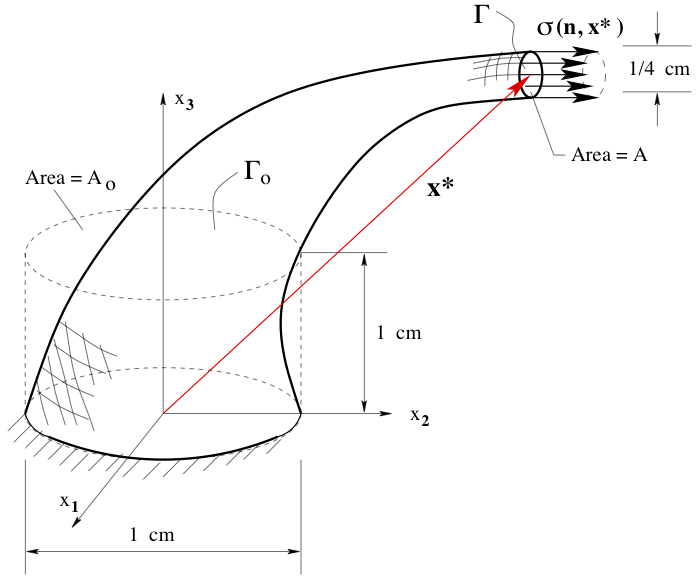
\includegraphics[width=0.7\textwidth]{RubberPlug.png}
% RubberPlug.png: 698x584 pixel, 150dpi, 11.82x9.89 cm, bb=0 0 335 280
\caption{Illustrative sketch of the rubber plug.}
\end{figure}

\subsubsection*{Solution}
From our limited amount of information, we know that $\mathbf{p}_0$ must be in
the $\mathbf{e}_3$ direction with a value such that the total force on the face
of the reference configuration matches the total force on the current
configuration. Therefore, let $F_s$ denote the total scalar value of force on
the face. Then on the current configuration,
\[
F_s=1000\,\frac{\text{kg}}{\text{cm}^2}\left(\frac{\pi}{4}(.25\,\text{cm}
)^2\right)=49.087\,\text{kg}\,.
\]
We know that $\mathbf{p}_0$ is uniform on $\Gamma_0$, therefore
\[
\mathbf{p}_0=\frac{49.087\,\text{kg}}{\frac{\pi}{4}(1\,\text{cm})^2}\mathbf{e}
_3=62.5\mathbf{e}_3\,\frac{\text{kg}}{\text{cm}^2}
\]
We have very limited knowledge of the stress tensor, but there are a few things
that we can discern from the given information and schematic. We can gather
that $T_{22}(\mathbf{x}^*)=1000$. Also, since there is no motion in the $x_1$
direction, the first column must be zeros. Also, we know that the stress at
$\mathbf{x}^*$ is normal to the face, therefore $T_{12}=T_{32}=0$. There may be
vertical shear stresses at the face, so we will denote the third column entries
with anonymous $\cdot$'s. Therefore
\[
\mathbf{T}(\mathbf{x}^*)=\left[
% use packages: array
\begin{array}{ccc}
0 & 0 & \cdot \\
0 & 1000 & \cdot \\
0 & 0 & \cdot
        \end{array}
\right]\,.
\]
Furthermore, we know that
$\mathbf{P}(\mathbf{X})=\mathbf{T}(\mathbf{x})\Cof\mathbf{F}(\mathbf{X})$, and
$P_{23}=62.5$. Therefore $\Cof\mathbf{F}$ should scale $\mathbf{T}$ by $1/16$
and flip the second and third columns. Again, the first column doesn't really
matter
because there is no motion in that direction. Therefore, one possible tensor
for this situation is
\[
\Cof\mathbf{F}(X_1,X_2,1)=\left[
% use packages: array
\begin{array}{ccc}
1 & \cdot & 0 \\
0 & \cdot & 1/16 \\
0 & \cdot & 0
        \end{array}
\right]\,.
\]

\end{document}

